\subsection{Análisis competitivo}
\label{ch:competencias}

Esta sección posiciona a ImprontIA frente al \textit{proctoring} audiovisual y la biometría conductual educativa relevados en las secciones anteriores del estado del arte, mediante la estrategia del océano azul y sus dos herramientas: la \textbf{Matriz ERIC} (Eliminar, Reducir, Incrementar, Crear) y la \textbf{Curva de Valor}. El posicionamiento resultante es deliberadamente complementario, no sustitutivo: ImprontIA renuncia a la observación audiovisual del entorno físico para priorizar la amplitud de señales digitales, la explicabilidad y la revisión humana.

\subsubsection{Enfoque competitivo y base del análisis}

El análisis competitivo de ImprontIA parte de la comparación de referencia (\textit{benchmark}) desarrollada en el Estado del Arte (Tabla~\ref{tab:comparacion_enfoques}), y utiliza esa evidencia como base para explicitar una estrategia de diferenciación mediante la Matriz ERIC y la Curva de Valor.

ImprontIA se propone como una capa complementaria de trazabilidad del proceso de resolución basada en señales de interacción digital, contextualización, explicabilidad y revisión humana. Como renuncia deliberada, prescinde de la observación del entorno físico mediante cámara o micrófono, sin que esa renuncia implique una superioridad general en privacidad o invasividad: el \textit{User Research} (Capítulo~\ref{ch:user_research}) muestra que la percepción de invasividad no depende únicamente del mecanismo utilizado, sino también de qué se captura, con qué finalidad y bajo qué condiciones se comunica.

\subsubsection{Estrategia del océano azul}
\label{sec:oceano_azul}

La estrategia del océano azul distingue dos tipos de espacio de mercado~\parencite{KimMauborgne2005}. Los océanos rojos son las industrias existentes, con fronteras y reglas de competencia aceptadas, en las que las empresas compiten por una demanda dada mejorando los mismos atributos que sus rivales. Los océanos azules son espacios todavía no disputados, que se crean mediante innovación en valor: en lugar de elegir entre diferenciarse o reducir costos, se replantean los factores que la industria da por sentados, eliminando o reduciendo algunos e incrementando o creando otros, para ofrecer un valor distinto a quien decide y a quien usa el producto.

En la supervisión de evaluaciones digitales, el \textit{proctoring} audiovisual se comporta como un océano rojo: sus productos compiten por ofrecer más observación del entorno físico, más restricciones del entorno digital y más alertas automáticas (Sección~\ref{ch:estado_arte}). ImprontIA compite en un espacio distinto: la trazabilidad del proceso de resolución, la interpretación de los eventos según las reglas de cada evaluación, la explicabilidad de cada indicador y el panorama agregado para el docente. La Matriz ERIC (Sección~\ref{sec:eric}) explicita qué factores se eliminan, reducen, incrementan y crean, y la Curva de Valor (Sección~\ref{sec:curva_valor}) representa el perfil resultante frente a las alternativas. Este posicionamiento es una hipótesis estratégica: la existencia efectiva de ese espacio de mercado requiere validarse con instituciones y docentes.

\subsubsection{Matriz ERIC}
\label{sec:eric}

La Matriz ERIC (Eliminar, Reducir, Incrementar, Crear), herramienta de la estrategia del océano azul~\parencite{KimMauborgne2005}, sintetiza las prioridades y renuncias de la propuesta frente al \textit{proctoring} audiovisual y la biometría conductual educativa relevados en el estado del arte. El cuadrante Crear refiere a elementos incorporados dentro de la propuesta de valor de ImprontIA y no a afirmaciones de novedad mundial.

\begin{table}[h!]
    \caption{Matriz ERIC de ImprontIA}
    \label{tab:matriz_eric}
    \centering
    \small
    \begin{tabularx}{\textwidth}{X X}
        \toprule
        \rowcolor{accent!15}\textbf{ELIMINAR} & \textbf{REDUCIR} \\
        \midrule
        \begin{minipage}[t]{\linewidth}
        \begin{itemize}[leftmargin=1em]
            \item Captura audiovisual del entorno físico como parte de la propuesta de ImprontIA.
            \item Dependencia del bloqueo del navegador o de la interrupción automática como mecanismo central de control.
            \item Decisiones académicas automáticas derivadas directamente de señales o indicadores.
        \end{itemize}
        \end{minipage}
        &
        \begin{minipage}[t]{\linewidth}
        \begin{itemize}[leftmargin=1em]
            \item Dependencia de una única modalidad o señal para interpretar una sesión.
            \item Alcance de la recolección a las señales necesarias y previamente definidas para cada evaluación.
            \item Interferencia del mecanismo de supervisión sobre el desarrollo normal de la evaluación.
        \end{itemize}
        \end{minipage} \\
        \addlinespace[6pt]
        \rowcolor{accent!15}\textbf{INCREMENTAR} & \textbf{CREAR} \\
        \midrule
        \begin{minipage}[t]{\linewidth}
        \begin{itemize}[leftmargin=1em]
            \item Amplitud de señales de interacción digital utilizadas para comprender la sesión.
            \item Contextualización académica de las señales e indicadores.
            \item Explicabilidad y trazabilidad entre indicador y evidencia de origen.
            \item Centralidad de la revisión humana antes de una valoración académica.
        \end{itemize}
        \end{minipage}
        &
        \begin{minipage}[t]{\linewidth}
        \begin{itemize}[leftmargin=1em]
            \item Una capa complementaria de trazabilidad del proceso de resolución.
            \item Una lectura integrada de señales de interacción digital y contexto académico.
            \item Un flujo explícito indicador \texorpdfstring{$\rightarrow$}{->} revisión humana \texorpdfstring{$\rightarrow$}{->} validación adicional cuando corresponda.
        \end{itemize}
        \end{minipage} \\
        \bottomrule
    \end{tabularx}
\end{table}

\subsubsection{Curva de Valor}
\label{sec:curva_valor}

La Curva de Valor, trazada sobre el cuadro estratégico~\parencite{KimMauborgne2005}, compara \textit{proctoring} audiovisual, biometría conductual educativa e ImprontIA sobre cuatro factores para los que el \textit{benchmark} del estado del arte permite una comparación defendible. La codificación Bajo~=~1, Medio~=~2 y Alto~=~3 se emplea únicamente con fines de representación visual; los niveles representan énfasis relativo de cada enfoque según el \textit{benchmark} analizado y no métricas de desempeño, precisión o calidad.

\begin{figure}[h!]
    \centering
    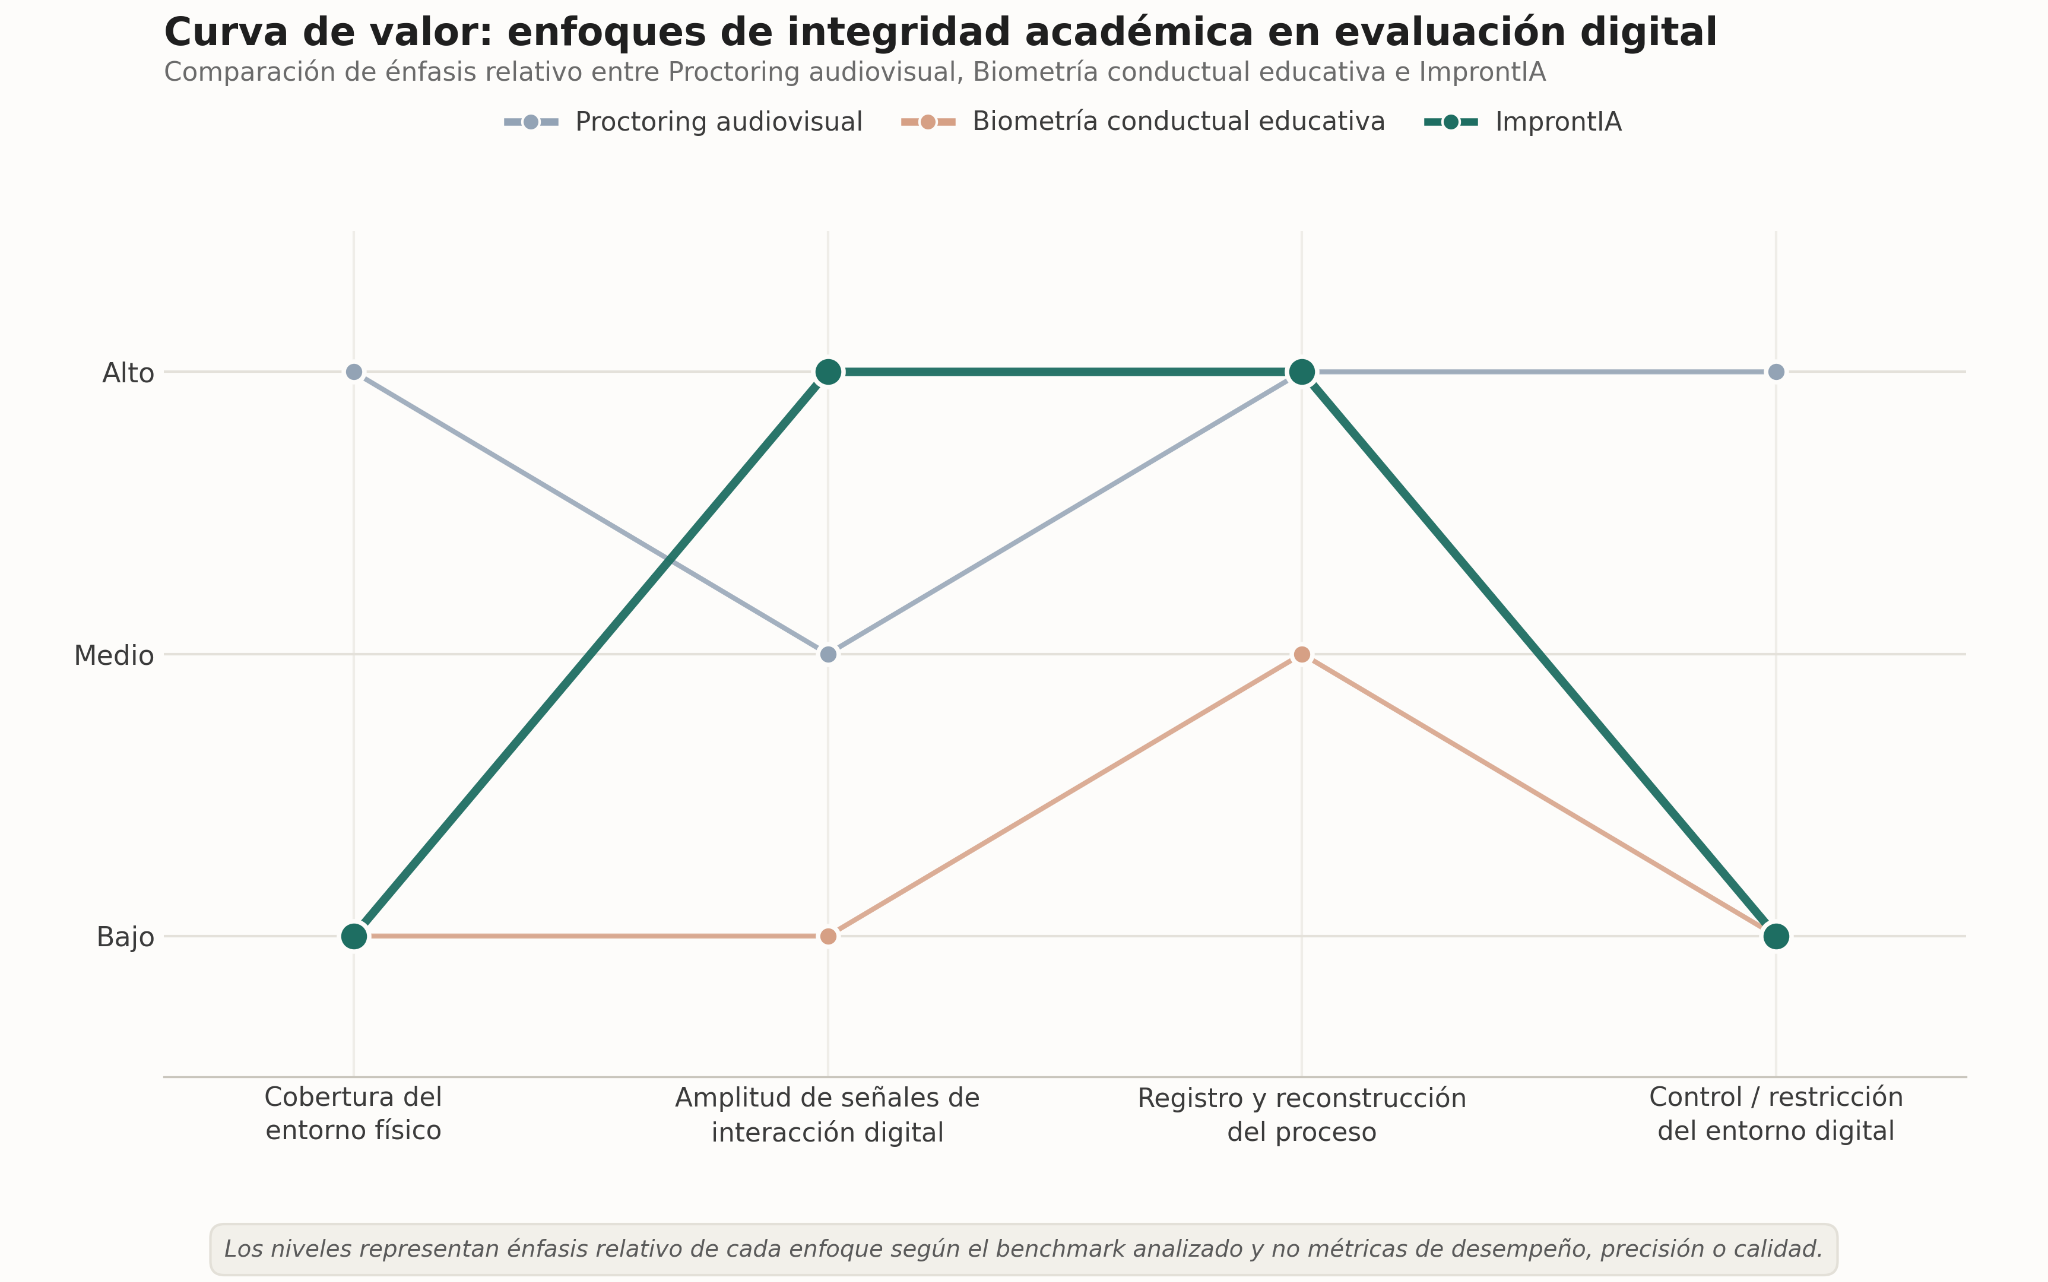
\includegraphics[width=0.95\textwidth]{./figures/competencias_curva_valor}
    \caption[Curva de Valor de ImprontIA frente a los enfoques comparados]{Curva de Valor de ImprontIA frente a los enfoques comparados. Fuente: elaboración propia a partir del \textit{benchmark} del estado del arte, sobre el cuadro estratégico de \textcite{KimMauborgne2005}.}
    \label{fig:curva_valor}
\end{figure}

\begin{table}[h!]
    \caption{Factores comparados en la Curva de Valor}
    \label{tab:curva_valor}
    \centering
    \small
    \begin{tabularx}{\textwidth}{X c c c}
        \toprule
        \tblhead \textbf{Factor} & \textbf{\textit{Proctoring} audiovisual} & \textbf{Biometría conductual educativa} & \textbf{ImprontIA} \\
        \midrule
        Cobertura del entorno físico & Alto (3) & Bajo (1) & Bajo (1) \\
        Amplitud de señales de interacción digital & Medio (2) & Bajo (1) & \textbf{Alto (3)} \\
        Registro y reconstrucción del proceso durante la sesión & Alto (3) & Medio (2) & \textbf{Alto (3)} \\
        Control / restricción del entorno digital & Alto (3) & Bajo (1) & Bajo (1) \\
        \bottomrule
    \end{tabularx}
\end{table}

\subsubsection{Síntesis de posicionamiento y renuncias}

La comparación muestra perfiles estratégicos diferentes y evita plantear una superioridad general de ImprontIA. El \textit{proctoring} audiovisual presenta mayor énfasis en la observación del entorno físico y en mecanismos de control o restricción del entorno digital, capacidades a las que ImprontIA renuncia deliberadamente. La biometría conductual educativa concentra su propuesta en un conjunto más acotado de señales, mientras que ImprontIA prioriza la amplitud de señales de interacción digital y la reconstrucción del proceso desarrollado durante la sesión.

Sobre esa base, ImprontIA incorpora como ejes de su propuesta la contextualización académica, la explicabilidad del vínculo entre indicadores y evidencia y la revisión humana. Estos factores no se incorporan a la Curva de Valor porque el \textit{benchmark} disponible no permite asignar niveles comparativos suficientemente rigurosos a las otras categorías en esas dimensiones.

\begin{keyfinding}{Posicionamiento resultante}
ImprontIA se posiciona como una capa \textbf{complementaria} ---no sustitutiva--- que aporta trazabilidad del proceso dentro del entorno digital, y mantiene separadas la generación de un indicador, la interpretación docente y una eventual validación adicional cuando corresponda.
\end{keyfinding}
